% Desenvolvido por Prof. Dr. David Buzatto
%
% Baseado na documentação do abntex2 e nos modelos em
% Microsoft Word propostos pela Profa. Dra. Rosana F. L. Rodrigues
% e pela bibliotecária M.Sc. Maria Carolina Gonçalves do campus
% São João da Boa Vista do IFSP.
%
% Versão 1.3
% Data: 09/08/2018

\documentclass[
	% -- opções da classe memoir --
	12pt,				% tamanho da fonte
	oneside,			% impressão em um lado
	a4paper,			% tamanho do papel. 
	%normalfigtabnum,
	%pnumromarab,
	% -- opções da classe abntex2 --
	chapter=TITLE,		% títulos de capítulos convertidos em letras maiúsculas
	section=TITLE,		% títulos de seções convertidos em letras maiúsculas
	%subsection=TITLE,	% títulos de subseções convertidos em letras maiúsculas
	%subsubsection=TITLE,% títulos de subsubseções convertidos em letras maiúsculas
	% -- opções do pacote babel --
	english,			% idioma adicional para hifenização
	french,				% idioma adicional para hifenização
	spanish,			% idioma adicional para hifenização
	brazil,				% o último idioma é o principal do documento
]{abntex2}






% ---------------------------------------------------------------------------------
%                                   PACOTES
% ---------------------------------------------------------------------------------

% ---
% Pacotes básicos 
% ---
\usepackage{lmodern}			% Usa a fonte Latin Modern			
\usepackage[T1]{fontenc}		% Selecao de codigos de fonte.
\usepackage[utf8]{inputenc}		% Codificacao do documento (conversão automática dos acentos)
\usepackage{lastpage}			% Usado pela Ficha catalográfica
\usepackage{indentfirst}		% Indenta o primeiro parágrafo de cada seção.
\usepackage{color}				% Controle das cores
\usepackage{graphicx}			% Inclusão de gráficos
\usepackage{microtype} 			% para melhorias de justificação
\usepackage{hyperref}
\usepackage{subfig}
\usepackage{epigraph}
\usepackage{url}
\usepackage{placeins}
\usepackage{multirow}
\usepackage[figuresright]{rotating}
\usepackage{chemfig}
\usepackage{amsmath}
\usepackage{amssymb}
\usepackage{enumitem}
\usepackage{bigints}
\usepackage{listings}
\usepackage{tabularx}
\usepackage{booktabs}
\usepackage{lastpage}
\usepackage{etoolbox}
% ---

% ---
% Pacotes adicionais, usados apenas no âmbito do Modelo Canônico do abnteX2
% ---
\usepackage{lipsum}				% para geração de dummy text
% ---

% ---
% Pacotes de citações
% ---
\usepackage[brazilian,hyperpageref]{backref}	 % Paginas com as citações na bibl
\usepackage[alf,abnt-emphasize=bf]{abntex2cite}  % Citações padrão ABNT


% ---------------------------------------------------------------------------------
%                          CONFIGURAÇÕES DOS PACOTES
% ---------------------------------------------------------------------------------

% ---
% Configurações do pacote backref
%
% Para desativar, tire o comentário de \begin{comment} e \end{comment} 
% das próximas linhas e comente a linha \usepackage[brazilian,hyperpageref]{backref}
% acima.
% ---

%\begin{comment}
% ---
% Configurações do pacote backref
% Usado sem a opção hyperpageref de backref
\renewcommand{\backrefpagesname}{Citado na(s) página(s):~}
% Texto padrão antes do número das páginas
\renewcommand{\backref}{}
% Define os textos da citação
\renewcommand*{\backrefalt}[4]{
	\ifcase #1 %
	Nenhuma citação no texto.%
	\or
	Citado na página #2.%
	\else
	Citado #1 vezes nas páginas #2.%
	\fi}%
% ---
%\end{comment}


% listagens
\definecolor{corComentario}{RGB}{150,150,150}
\definecolor{corString}{RGB}{206,123,0}
\definecolor{corPalavraChave}{RGB}{0,0,230}

\lstset{
	numbers=left,
	stepnumber=1,
	firstnumber=1,
	numberstyle=\footnotesize,
	extendedchars=true,
	breaklines=true,
	lineskip=0pt,
	frame=tb,
	basicstyle=\ttfamily\footnotesize,
	showstringspaces=false,
	stringstyle=\color{corString},
	commentstyle=\color{corComentario},
	keywordstyle=\color{corPalavraChave}
}

\newcolumntype{Y}{>{\centering\arraybackslash}X}

\newcommand{\ano}[1]{\def \oano {#1}}
\newcommand{\imprimirano}{\oano}

\newcommand{\mes}[1]{\def \omes {#1}}
\newcommand{\imprimirmes}{\omes}

\newcommand{\subtitulo}[1]{\def \osubtitulo {#1}}
\newcommand{\imprimirsubtitulo}{\osubtitulo}

\newcommand{\area}[1]{\def \aarea {#1}}
\newcommand{\imprimirarea}{\aarea}

\renewcommand{\coorientador}[1]{\def \ocoorientador {#1}}
\renewcommand{\imprimircoorientador}{\ocoorientador}

\newcommand{\grau}[1]{\def \ograu {#1}}
\newcommand{\imprimirgrau}{\ograu}

\newcommand{\curso}[1]{\def \ocurso {#1}}
\newcommand{\imprimircurso}{\ocurso}


% ---
% Informações de dados para CAPA e FOLHA DE ROSTO
% ---

\curso{Nome do Curso}
\grau{Definição do grau}

%exemplos
%\curso{Tecnologia em Sistemas para Internet}
%\grau{Tecnólogo em Sistemas para Internet}
%\curso{Especialização em Desenvolvimento de Aplicações para Dispositivos Móveis}
%\grau{Especialista em Desenvolvimento de Aplicações para Dispositivos Móveis}

\titulo{Título}

% caso não haja subtítulo, comente a linha abaixo
\subtitulo{subtítulo}

\tipotrabalho{Relatório Técnico}
\area{Área de Concentração do Trabalho}

\autor{Nome Completo}
\orientador{Prof./Profa. Me./Dr./Dra. Nome Completo}

% caso não haja coorientador, comente a linha abaixo
\coorientador{Prof./Profa. Me./Dr./Dra. Nome Completo}

\local{São João da Boa Vista}
\mes{MÊS}
\ano{ANO}

\instituicao{%
	Instituto Federal de Educação, Ciência e Tecnologia de São Paulo
	\par
	Câmpus São João da Boa Vista
}

\preambulo{\imprimirtipotrabalho\ elaborado conforme a ABNT NBR 10719:10, apresentado ao Instituto Federal de Educação, Ciência e Tecnologia de São Paulo, como parte dos requisitos para a obtenção do grau de \imprimirgrau.
\\
\\
Área de Concentração: \imprimirarea}
% ---


% ---
% Configurações de aparência do PDF final
% ---

% alterando o aspecto da cor azul
\definecolor{blue}{RGB}{41,5,195}

% informações do PDF
\makeatletter
\hypersetup{
	%pagebackref=true,
	pdftitle={\@title}, 
	pdfauthor={\@author},
	pdfsubject={\imprimirpreambulo},
	pdfcreator={Nome Completo},
	pdfkeywords={Palavra chave 1}{Palavra chave 2}{Palavra chave 3}{Palavra chave n}, 
	colorlinks=true,       		% false: boxed links; true: colored links
	linkcolor=black,          	% color of internal links
	citecolor=black,       		% color of links to bibliography
	filecolor=black,      		% color of file links
	urlcolor=black,
	bookmarksdepth=4
}
\makeatother
% --- 


% ---
% Comandos do autor
% ---

% comando para inserir autor e ano
\newcommand{\citeauthorandyear}[1]{\citeauthoronline{#1} (\citeyear{#1})}


% ---
% Novo list of (listings) para Quadros
% ---

\newcommand{\quadroname}{Quadro}
\newcommand{\listofquadrosname}{Lista de Quadros}

\newfloat[chapter]{quadro}{loq}{\quadroname}
\newlistof{listofquadros}{loq}{\listofquadrosname}
\newlistentry{quadro}{loq}{0}

% configurações para atender às regras da ABNT
\setfloatadjustment{quadro}{\centering}
\counterwithout{quadro}{chapter}
\renewcommand{\cftquadroname}{\quadroname\space} 
\renewcommand*{\cftquadroaftersnum}{\hfill--\hfill}

% Configuração de posicionamento padrão:
\setfloatlocations{quadro}{hbtp}



% --- 
% Espaçamentos entre linhas e parágrafos 
% --- 

% O tamanho do parágrafo é dado por:
\setlength{\parindent}{1.3cm}

% Controle do espaçamento entre um parágrafo e outro:
\setlength{\parskip}{0.2cm}  % tente também \onelineskip

% ---
% compila o indice
% ---
\makeindex
% ---







% ---------------------------------------------------------------------------------
%                                   INÍCIO DO DOCUMENTO
% ---------------------------------------------------------------------------------
\begin{document}

% Seleciona o idioma do documento (conforme pacotes do babel)
%\selectlanguage{english}
\selectlanguage{brazil}

% Retira espaço extra obsoleto entre as frases.
\frenchspacing 

\pretextual
\begin{center}
   	
   	\ABNTEXchapterfont\Large\textsc{\imprimirautor}
   	\vspace{2.5cm}
   	
   	\ABNTEXchapterfont\LARGE\textsc{\imprimirtitulo\ifdef{\osubtitulo}{:}{}}

    \ifdef{\osubtitulo}{\ABNTEXchapterfont\Large\imprimirsubtitulo}{}
   	\vspace{2.5cm}
   	   	
   	\hspace{.4\textwidth}
   	\begin{minipage}{.5\textwidth}
   		\SingleSpacing
   		\large\imprimirpreambulo
   		
   		\vspace{\onelineskip}
   		
   		Orientador: \imprimirorientador
   		
        \ifdef{\ocoorientador}{
            \vspace{\onelineskip}
               		
       		Coorientador: \imprimircoorientador
        }{}
        
        
   		
   	\end{minipage}%
    \vfill
   	
   	\Large\textsc{\imprimirlocal}
   	
   	\Large\textsc{\imprimirano}
   	
   	\vspace*{2cm}
   	
\end{center}
\newcommand{\specialcell}[2][c]{%
	\begin{tabular}[#1]{@{}c@{}}#2\end{tabular}}

\FloatBarrier
\begin{table}[!htbp]
	\centering
	\renewcommand{\arraystretch}{1.5}% Spread rows out...
	\begin{tabular}{| >{\centering}m{2in} | >{\centering}m{2in} | >{\centering\arraybackslash}m{2in} | }
		\hline
		\specialcell[t]{INSTITUTO FEDERAL DE\\EDUCAÇÃO, CIÊNCIA E\\TECNOLOGIA DE SÃO\\PAULO - CÂMPUS SÃO\\JOÃO DA BOA VISTA} & \imprimirmes & \imprimirano \\
		\hline
		\multicolumn{3}{|c|}{\specialcell{
				
				\\ \\
				
				\imprimircurso
				
				\\ \\ \\ \\ \\ \\
				
				\begin{minipage}[t]{0.9\columnwidth}%
				    \centering
				    \ABNTEXchapterfont\LARGE\imprimirtitulo\ifdef{\osubtitulo}{:}{}
                    
                    \ifdef{\osubtitulo}{\ABNTEXchapterfont\Large\imprimirsubtitulo}{}
                    
				\end{minipage}
				
				\\ \\ \\ \\
				
				}}\\
		\multicolumn{3}{|r|}{\specialcell{
				
                \begin{minipage}[t]{0.9\columnwidth}%
   				    \flushright
    				\imprimirautor \ifdef{\ocoorientador}{,}{\ e}
                    \\
                    \imprimirorientador \ifdef{\ocoorientador}{ e\\\imprimircoorientador}{}
                \end{minipage}
				
				\\ \\ \\ \\ \\ \\ \\ \\ \\ \\ 
				
			}}\\
			\hline
		\multicolumn{2}{|l|}{\specialcell{Palavras-chave:\\Palavra-chave 1. Palavra-chave 2. Palavra-chave n.}} & \the\numexpr \getpagerefnumber{LastPage} - 1 \relax \  páginas \\
		\hline
	\end{tabular}
\end{table}
\FloatBarrier


% ---
% inserir o sumário
% ---
\pdfbookmark[0]{\contentsname}{toc}
\tableofcontents*
\cleardoublepage
% ---

\chapter*{}
\noindent{\textbf{RESUMO}}

\noindent{Neste trabalho é apresentada a formatação que deve ser utilizada nos relatórios técnicos a serem submetidos ao final dos cursos de Graduação e Pós-graduação do IFSP câmpus São João da Boa Vista. Leia com atenção este documento. O máximo de palavras para o resumo é 150 (cento e cinquenta).}

\vspace{\onelineskip}

\noindent{\textbf{Palavras-chave}: Palavra-chave 1. Palavra-chave 2. Palavra-chave 3. Palavra-chave n.}

\textual
\chapter{Introdução}
\label{cap:01}

Parte inicial do texto, na qual devem constar o tema e a delimitação do assunto tratado, objetivos da pesquisa e outros elementos necessários para situar o tema do trabalho, tais como: justificativa, procedimentos metodológicos e estrutura do trabalho, tratados de forma sucinta. Salienta-se que os procedimentos metodológicos e o embasamento teórico são tratados, posteriormente, em capítulos próprios e com a profundidade necessária ao trabalho de pesquisa.

Neste documento estão listadas as seções obrigatórias que você deverá fornecer, bem como os exemplos dos comandos mais comuns que serão utilizados na construção de seu documento. Para pesquisar sobre mais comandos, recomenda-se a utilização do site \url{https://ctan.org/}, que é a biblioteca principal do \LaTeX, e o do site \url{https://tex.stackexchange.com} que é uma das principais comunidades para solução de dúvidas relacionadas a \LaTeX. Ambas são em inglês.

\section{Justificativa}

Texto da justificativa.

\section{Objetivos}

\subsection{Objetivo Geral}

Qual seu objetivo geral.

\subsection{Objetivos Específicos}
\begin{itemize}
	\item Objetivo específico 1;
	\item Objetivo específico 2;
	\item Objetivo específico n.
\end{itemize}



\section{Organização Deste Trabalho}

Como seu trabalho está organizado (capítulos).
\chapter{Considerações Gerais}
\label{cap:02}

Texto das considerações gerais, dividido em subseções.

Este é um exemplo de como usar figuras. Referência cruzada: Figura~\ref{fig:exemplo}

\FloatBarrier
\begin{figure}[!htbp]
	\centering
	\caption{Exemplo de figura}
	%scale redimensiona a figura.
	%1.5 = 150% do tamanho original
	%1 = 100% do tamanho original
	%0.20 = 20% do tamanho original
	
\includegraphics[scale=1.5]{imagens/exemploFigura}
	\\\textbf{Fonte:} Elaborada pelo autor
	\label{fig:exemplo}
\end{figure}
\FloatBarrier


Este é um exemplo de como usar tabelas. Referência cruzada: Tabela~\ref{tab:exemplo}

\FloatBarrier
\begin{table}[!htbp]
	\centering
	\caption{Exemplo de tabela de 2 colunas}
	\begin{tabular}{ c | c }
		\hline
		\textbf{Coluna 1} & \textbf{Coluna 2} \\ \hline
		Dado 1a           & Dado 1b           \\ \hline
		Dado 2a           & Dado 2b           \\ \hline
		Dado 3a           & Dado 3b           \\ \hline
		Dado 4a           & Dado 4b           \\ \hline
	\end{tabular}
	\\ \vspace{0.2cm}
	\textbf{Fonte:} Elaborada pelo autor
	\label{tab:exemplo}
\end{table}
\FloatBarrier


Este é um exemplo de como usar quadros. Referência cruzada: Quadro~\ref{qua:exemplo}

\FloatBarrier
\begin{quadro}[!htbp]
	\centering
	\caption{Exemplo de quadro}
	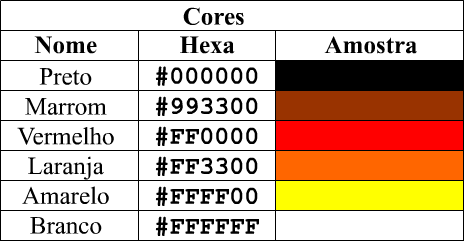
\includegraphics[scale=.7]{imagens/exemploQuadro}
	\\\textbf{Fonte:} Elaborada pelo autor
	\label{qua:exemplo}
\end{quadro}
\FloatBarrier


Este é um exemplo de como usar equações. Referência cruzada: Equação~\ref{eq:exemplo}

\begin{equation}
\sum_{i=1}^{n} = \frac{n(n+1)}{2}
\label{eq:exemplo}
\end{equation}


Exemplo de inserção de lista de código fonte (\textbf{\textcolor{red}{não use acentos no código!}}):

\lstinputlisting[language=Java]{fontes/ClasseExemplo.java} 



Este é um exemplo de como inserir texto sem formatação (ambiente verbatim):

\begin{verbatim}
Texto sem formatação, como espaçamento igual.
\end{verbatim}


Exemplo de lista de itens:

\begin{itemize}
	\item \textbf{Item 1:} texto...;
	\item \textbf{Item 2:} texto...;
    \begin{itemize}
            \item \textbf{Subitem:} texto...;
            \item \textbf{Subitem:} texto...;
            \item \textbf{Subitem:} texto...;
        \end{itemize}
	\item \textbf{Item 3:} texto...;
	\item \textbf{Item n:} texto....
\end{itemize}


Exemplo de lista numerada:

\begin{enumerate}
	\item \textbf{Item:} texto...;
	\item \textbf{Item:} texto...;
    \begin{enumerate}
        \item \textbf{Subitem:} texto...;
        \item \textbf{Subitem:} texto...;
        \item \textbf{Subitem:} texto...;
    \end{enumerate}
	\item \textbf{Item:} texto...;
	\item \textbf{Item:} texto....
\end{enumerate}


Exemplos de comandos para texto e referências:

\begin{itemize}
	\item Para iniciar um novo parágrafo, basta deixar uma linha em branco no código fonte;
	\item Não force o compilador a pular mais de uma linha, pois terá influência negativa na composição do documento;
	\item Sempre deixe o \LaTeX\ realizar a formatação de parágrafos e posicionamento de elementos;
	\item Utilização de aspas simples (abertura \verb|`|, fechamento \verb|'|): `Texto entre aspas simples';
	\item Utilização de aspas duplas (abertura \verb|``|, fechamento \verb|''|): ``Texto entre aspas duplas'';
	\item Negrito (comando \verb|\textbf|): \textbf{texto em negrito};
	\item Itálico (comando \verb|\textit|): \textit{texto em itálico};
	\item Sublinhado (comando \verb|\underline|): \underline{texto sublinhado};
	\item Negrito e itálico (usar comandos juntos): \textbf{\textit{texto em negrito e itálico}};
	\item Alterar cor do texto (comando \verb|\textcolor{cor}{texto}|):
	\begin{itemize}
		\item Exemplo \verb|\textcolor{red}{texto}|: \textcolor{red}{texto vermelho};
		\item Exemplo \verb|\textcolor[RGB]{255, 102, 0}|: \textcolor[RGB]{255, 102, 0}{texto laranja};
		\item Exemplo \verb|\textcolor[HTML]{006AD7}|: \textcolor[HTML]{006AD7}{texto azul};
	\end{itemize}
	\item Ambiente matemático inline (comando \verb|$ expressão $|): $s = x^2-2x +1$;
	\item Referência normal (comando \verb|\cite|):
	\begin{itemize}
		\item \cite{Agaisse1995};
		\item \cite{Abedi2014};
		\item \cite{BtNomenclature2016};
	\end{itemize}
	\item Referência normal com mais de uma obra (comando \verb|\cite|):
	\begin{itemize}
		\item \cite{Agaisse1995, Abedi2014};
		\item \cite{Nelson2014, BtNomenclature2016, AgapitoTenfen2014};
	\end{itemize}
	\item Referência nome e ano (comando \verb|\citeauthorandyear|):
	\begin{itemize}
		\item \citeauthorandyear{Agaisse1995};
		\item \citeauthorandyear{Abedi2014};
		\item \citeauthorandyear{BtNomenclature2016};
	\end{itemize}
\end{itemize}


Exemplo 1 de referência direta:

\begin{citacao}
	Os 20 aminoácidos usualmente encontrados como resíduos em proteínas contém um grupo $\alpha$-carboxil, um grupo $\alpha$-amino e um grupo R distinto substituído no átomo de carbono $\alpha$. O átomo de carbono $\alpha$ de todos os aminoácidos, com exceção da glicina, é assimétrico e, portanto, os aminoácidos podem existir em pelo menos duas formas estereoisoméricas. Somente os estereoisômeros L, com uma configuração relacionada à configuração absoluta da molécula de referência L-gliceraldeído, são encontrados em proteínas \cite[p. 81]{Nelson2014}
\end{citacao}

Exemplo 2 de referência direta:

\begin{citacao}
	\textit{These various insecticidal proteins are synthesized during the stationary phase and accumulate in the mother cell as a crystal inclusion which can account for up to 25\% of the dry weight of the sporulated cells. The amount of crystal protein produced by a B. thuringiensis culture in laboratory conditions (about 0.5 mg of protein per ml) and the size of the crystals (24) indicate that each cell has to synthesize $10^6$ to $2 \times 10^6$ $\delta$-endotoxin molecules during the stationary phase to form a crystal} \cite[p. 1]{Agaisse1995}
\end{citacao}

Exemplo de nota de rodapé\footnote{Essa é uma nota de rodapé!}.

\chapter{Metodologia}
\label{cap:03}

Descrever metodologia, materiais e métodos utilizados no estudo, bem como os procedimentos experimentais realizados (equipamentos, técnicas e processos utilizados).

\chapter{Análise dos Resultados}
\label{cap:04}

Relatar os resultados obtidos a partir dos experimentos e dos estudos realizados. 


\section{Resultados/Impactos}

Resultados


\section{Orçamento}

Orçamento, caso exista


\section{Cronograma do trabalho}

Cronograma

\chapter{Conclusões e Recomendações}
\label{cap:05}

São   descritas   claramente   as   conclusões retiradas   das discussões  e  dos  experimentos  realizados  no  decorrer  da  pesquisa,  e  finalizada  a parte  textual  do  trabalho.  Recomendações  são  declarações  concisas  de  ações, julgadas necessárias a partir das conclusões obtidas, a serem usadas no futuro.


% ----------------------------------------------------------
% Referências bibliográficas
% ----------------------------------------------------------
\postextual
\bibliography{referencias}


\end{document}
